% 复数

\pentry{几何矢量\upref{GVec}, 三角恒等式\upref{TriEqv}}
我们首先定义\bb{虚数单位} $\I$ 满足 $\I^2 = -1$, 则任何一个复数 $z$ 可以表示为\footnote{为了与变量 $i$ 区分, 本书中虚数单位使用正体的 $\I$.}
\begin{equation}
z = x + \I y
\end{equation}
其中 $x,y$ 为任意实数, 分别被称为复数 $z$ 的\bb{实部(real part)}和\bb{虚部(imaginary part)}, 记为 $\Re[z]$ 和 $\Im[z]$.

\begin{figure}[ht]
\centering
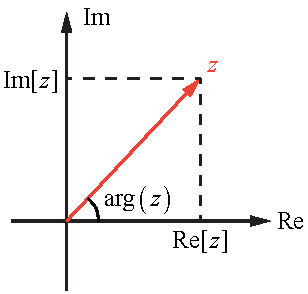
\includegraphics[width=4.7cm]{./figures/CplxNo1.pdf}
\caption{复平面与复数} \label{CplxNo_fig1}
\end{figure}

如\autoref{CplxNo_fig1}, 一个复数可以看做\bb{复平面}上的一个点(或矢量), 该矢量在复平面的\bb{实轴}和\bb{虚轴}方向的分量分别等于其实部和虚部. 复数的\bb{模长}定义为对应矢量的模长, 即
\begin{equation}
\abs{z} = \sqrt{\Re[z]^2 + \Im[z]^2}
\end{equation}
另外我们把矢量与实轴的夹角称为\bb{幅角}, 记为 $\arg(z)$. 我们可以通过实部和虚部计算幅角%未完成:这里应该用 arctan2,并链接到定义
\begin{equation}
\arg(z) = \arctan(\Im[z]/\Re[z])
\end{equation}
也可以通过模长和幅角来计算实部与虚部
\begin{equation}
\Re[z] = \abs{z}\cos(\arg z) \qquad \Im[z] = \abs{z}\sin(\arg z)
\end{equation}
在“指数函数(复数)\upref{CExp}” 中我们将看到, 任意复数也可以通过欧拉公式表示为以下形式
\begin{equation}
z = A(\cos\theta + \I\sin\theta) = A\E^{\I\theta}
\end{equation}
其中 $A = \abs{z}$, $\theta = \arg z$.

\subsection{基本运算}
\subsubsection{共轭}
一个复数的共轭等于一个实部相同,虚部相反的复数
\begin{equation}\label{CplxNo_eq6}
z\Cj = \Re[z] - \I \Im[z]
\end{equation}
所以共轭运算不改变复数的模长, 但将其幅角变为相反数.

\subsubsection{加和减}
复数的加减就是把两个复数的实部与虚部分别相加减(为了书写方便, 这里把复数 $z_i$ 的实部虚部记为 $x_i, y_i$)
\begin{equation}
z_1 \pm z_2 = (x_1 \pm x_2) + \I (y_1 \pm y_2)
\end{equation}
在复平面上, 这相当于把两个复数对应的矢量进行矢量相加减. 显然, 复数的加法满足交换律, 分配律和结合律.

特殊地, 将一个复数与其复共轭加减可得
\begin{equation}
\Re[z] = \frac12 (z + z\Cj) \qquad
\Im[z] = \frac12 (z - z\Cj)
\end{equation}

\subsubsection{乘法}
两个复数相乘定义为(注意应用 $\I^2 = -1$)
\begin{equation}
z_1z_2 = (x_1 + \I y_1)(x_2 + \I y_2) = (x_1 x_2 - y_1 y_2) + \I (x_1 y_2 + x_2 y_1)
\end{equation}
可以证明复数相乘后, 乘积的模长等于两复数模长之积, 乘积的幅角等于两复数的幅角之和, 即
\begin{align}
\abs{z_1 z_2} &= \abs{z_1}\abs{z_2}\\
\arg(z_1 z_2) &= \arg(z_1) + \arg(z_2)
\end{align}
证明如下: 令 $A_i = \abs{z_i}$, $\theta_i = \arg z_i$, 则
\begin{equation}\ali{
z_1 z_2 &= (A_1 \cos\theta_1 + \I A_1 \sin\theta_1)(A_2 \cos\theta_2 + \I A_2 \sin\theta_2)\\
&= A_1 A_2 (\cos\theta_1\cos\theta_2 - \sin\theta_1\sin\theta_2) + \I A_1 A_2 (\cos\theta_1\sin\theta_2 + \cos\theta_2\sin\theta_1)\\
&= A_1 A_2 [\cos(\theta_1 + \theta_2) + \I \sin(\theta_1 + \theta_2)]
}\end{equation}
其中最后一步用到了两角和公式\autoref{TriEqv_eq1}\upref{TriEqv}. 容易看出, 最后得到的是一个模长为 $A_1 A_2$, 幅角为 $\theta_1 + \theta_2$ 的复数.

不难证明复数的乘法满足交换律和结合律.

特殊地, 一个复数乘以其复共轭可得其模长的平方.
\begin{equation}
z z\Cj = x^2 + y^2 = \abs{z}^2
\end{equation}

\subsubsection{除法}
令 $z_1 = z z_2$, 则两个复数相除可以记为
\begin{equation}
z = \frac{z_1}{z_2} = \frac{x_1 + \I y_1}{x_2 + \I y_2}
\end{equation}
但我们希望可以将结果的实部与虚部分开, 于是我们可以在等式两边同时乘以 $z_2\Cj$, 即 $z_1 z_2\Cj  = z z_2 z_2\Cj$, 或
\begin{equation}
z = \frac{z_1 z_2\Cj}{z_2 z_2\Cj}
= \frac{(x_1 + \I y_1)(x_2 - \I y_2)}{(x_2 + \I y_2)(x_2 - \I y_2)}
= \frac{x_1 x_2 + y_1 y_2}{x_2^2 + y_2^2} + \I \frac{x_2 y_1 - x_1 y_2}{x_2^2 + y_2^2}
\end{equation}
这个步骤叫做\bb{分母有理化}.
